% REMEMBER: You must not plagiarise anything in your report. Be extremely careful.

\documentclass{l4proj}

    
%
% put any additional packages here
%

\begin{document}

%==============================================================================
%% METADATA
\title{Demonstrating the security of a basic cryptocurrency}
\author{Sean Horgan}
\date{September 14, 2018}

\maketitle

%==============================================================================
%% ABSTRACT
\begin{abstract}
    \vskip 0.5em
    Over the past decade, cryptocurrency has become a rapidly growing area of interest as it aims to provide a 
    decentrilised alternative to regular fiat currencies. The goal of this project is to implement a peer-based 
    cryptocurrency. It is designed to include a distributed, tamper-proof ledger, a consensus mechanism 
    for distributing transactions to all participating nodes, a mining system, and wallets for sending 
    the currency between different addresses. It also includes a test harness so that a number of nodes 
    can be created and run on a single computer in order to test the system.
\end{abstract}

%==============================================================================

% EDUCATION REUSE CONSENT FORM
% If you consent to your project being shown to future students for educational purposes
% then insert your name and the date below to  sign the education use form that appears in the front of the document. 
% You must explicitly give consent if you wish to do so.
% If you sign, your project may be included in the Hall of Fame if it scores particularly highly.
%
% Please note that you are under no obligation to sign 
% this declaration, but doing so would help future students.
%
\def\consentname {Sean Horgan} % your full name
\def\consentdate {12 November 2019} % the date you agree
%
\educationalconsent


%==============================================================================
\tableofcontents

%==============================================================================
%% Notes on formatting
%==============================================================================
% The first page, abstract and table of contents are numbered using Roman numerals and are not
% included in the page count. 
%
% From now on pages are numbered
% using Arabic numerals. Therefore, immediately after the first call to \chapter we need the call
% \pagenumbering{arabic} and this should be called once only in the document. 
%
% Do not alter the bibliography style.
%
% The first Chapter should then be on page 1. You are allowed 40 pages for a 40 credit project and 30 pages for a 
% 20 credit report. This includes everything numbered in Arabic numerals (excluding front matter) up
% to but excluding the appendices and bibliography.
%
% You must not alter text size (it is currently 10pt) or alter margins or spacing.
%
%
%==================================================================================================================================
%
% IMPORTANT
% The chapter headings here are **suggestions**. You don't have to follow this model if
% it doesn't fit your project. Every project should have an introduction and conclusion,
% however. 
%
%==================================================================================================================================
\chapter{Introduction}

% reset page numbering. Don't remove this!
\pagenumbering{arabic} 

\section{Motivation}

The concept of cryptocurrency has only emerged in the past fifteen years as an alternative to the regular,
centralised fiat currencies backed by governments around the world. In 2008 Satoshi Nakamoto, the 
founder of Bitcoin, invented the worlds first cryptocurrency providing a peer-to-peer currency
not bound to a central bank. This new currency, secured by modern cryptographic methods, is a way in
which people around the world can trade without having to send the funds via a financial institution. (REFERENCE).

This new currency ensured security to its users by implementing a distributed ledger of transactions. Bitcoin
ensured that the ledger was immutable by ensuring proof of work was given before transactions would be
added to this ledger. This invention, known as the blockchain, maintained security and prevented malicious
users from altering the system. Now the blockchain has become more than just a measure for ensuring security
in cryptocurrencies becoming useful to thousands of companies around the world and being used
in many different contexts.

Bitcoin and other cryptocurrencies are much different to current fiat currencies as they are not tied to a physical
object like a note or coin. They are also immune to inflation as the value of currency in the system is dictated
by the proof of work system. This rewards nodes for mining blocks of transactions with a small amount of the 
currency. As the currency ages this reward is reduced until eventually there won't be any more given. This places
a limit on the total amount of the currency available. 

\section{Goals}
The goal of this project is to create a secure and robust cryptocurrency from scratch. There are several key aspects
to the project that must be met in order to demonstrate a woking cryptocurrency.

The currency will be based around
a distributed ledger that is resistant to retroactive changes. It will use a concept know as proof of work,
similar to the way that Bitcoin works where nodes have to solve difficult hashing calculations in order
to add transactions to the ledger. This concept is known as mining and is a way to make sure that transactions
are added at a steady rate while providing compensation to the node as an incentive to verify the transactions the node
is trying to add are valid and acceptable.

This cryptocurrency will include wallets, allowing users to send any of their currency to another
wallet using its public key address. This will be shown in the test harness where a number of nodes and wallets 
will be created to simulate a populated network of users. A large number of emulated users will be required because on
a smaller scale cryptocurrencies do not work perfectly and are succeptable to double-spending attacks where users
can spend more money than they own. The test harness should simulate a large active network by randomly creating
transactions from user to user to then be added to the blockchain once the nodes have shown proof of work using 
the mining mechanism.

\section{Dissertation Outline}
The following dissertaiton is split into seven chapters as described below:
\begin{itemize}
    \item
        \textbf{Chapter 2} gives insight into the original Bitcoin paper and other features of cryptocurrencies
        created in the past.
    \item
        \textbf{Chapter 3} discusses the requirements gathering and analysis stage where the functionality
        of the project was decided.
    \item
        \textbf{Chapter 4} presents the way in which the cryptocurrency was designed, from the architecture of the blocks
        to the verification of transactions.
    \item
        \textbf{Chapter 5} highlights the way in which the projects was implemented, discussing the specific tools and 
        technologies used to create a secure cryptocurrency.
    \item
        \textbf{Chapter 6} discusses the evaluation of the projects. This shows how well the requirements were met, the
        performance of the system, and unit testing.
    \item
        \textbf{Chapter 7} concludes the project, summarising the project and reflecting on its execution. Here we also
        outline any future work that could be accomplished.
\end{itemize}


%==================================================================================================================================
\chapter{Background}
In this chapter we will discuss the background of the project. This will be presented by looking at the relevant research done by 
others that has similar goals to this project. We will also examine other cryptocurrencies created in the past that have aided 
in the completion of this project.


\section{Bitcoin white paper}
The first cryptocurrency to be created was Bitcoin. It was first presented in 2008 by Satoshi Nakamoto in the Bitcoin White Paper
titled "Bitcoin: A Peer-to-Peer Electronic Cash System". The concise nine page article defines Nakamoto's method of preventing
double-spending attacks in a peer-to-peer currency without the need for a third party like a financial institution to 
act as a middle man. The creater of Bitcoin wanted to avoid the use of a centralised mint as it can be seen as a single 
point of failure through which every transaction must be routed. This places the whole trust of the network on the middle 
man and the company running this mint.  Bitcoin avoids the need for a centralised middleman utilising modern cryptographic 
methods and technologies. This paper outlines the requirements for a functional cryptocurrency and as such was instrumental 
in guiding this project.

Below the main funtionality described in the Bitcoin white paper will be presented.


\subsection{Transactions}
The primary component of a cryptocurrency is a transaction between two users. In bitcoin this is described as being "a
chain of digital signatures". In this sense, a transaction is just a way of showing that ownership of the coin has
passed from the sender's address to the recipient's address. Bitcoin ensures the immutability of these transactions
by making the sender generate a hash of the previous transaction combined with the public key, equivalent to the address,
of the recipient. This means that the recipient can then verify the transaction using their own key and the transaction
is confirmed as valid.

One issue with this method is that the recipient can validate that the transaction is correct but it cannot ensure
that the sender is not double-spending the coin. This means the recipient cannot prevent the sender from also sending the 
same coin to another user. As Bitcoin was inteded to be a peer-to-peer currency with no centralised mint validating
all transactions and making sure there are no double spends, it is vital that there be some cryptographic method of
preventing these exploits.


\subsection{Blockchain}
The way Bitcoin achieves this validation without the need for a middleman is through the invention of the blockchain.
The blockchain is described as a timestamp server which works by taking the hash of a block of data and publically
announcing this hash. This proves that the data exists at that time. Then the next block of data can include the
previous block's hash in it's own hash proving that both of these blocks of data existed at that time. This creates 
a chain of blocks which prove the order and time of creation.

This chain of blocks is extremely secure as it also protects against retroactive attacks. If a malicious user tries
to go back and alter a transaction in the blockchain then this would alter the hash of that block rendering it invalid,
this would then alter the next block's hash as each block's hash is a calculation using the hash of the previous block.
This would cascade through the whole blockchain invalidating every block from the point of the malicious change. The 
network would then recognise this chain is invalid and switch to a valid chain rendering the action of the malicious
user pointless.

\subsection{Consensus}
In order for the whole system of users to work, all nodes must agree on what is the correct blockchain to be using and
which blocks of transactions are to be added to the blockchain every time. This is implemented by Bitcoin using a proof of
work mechanism. This system, also known as mining, means that in order for a node to add a block to the blockchain it
must find a value that, after being hashed, results in a number starting with a certain amount of '0's. This is 
effectivly setting a computational barrier to appending a block to the blockchain. This means that a certain amount of
CPU power is neseccary to append to the blockchain. This adds security to the system as it prevents singular malicious
users from hording IP addresses in order to take control of the network as theoretically the majority of computational
power in the network will be from benevolent users.


%***
It is easy for the nodes to decide which blockchain to add their blocks to because of this implementation of CPU power
determining which blocks are added to the blockchain. They simply choose the longest blockchain as this will be
the blockchain with the most CPU power invested in it. This is secure because if an attacker were trying to alter a 
previous block they would also have to redo all the proof of work completed for every block after that in the chain.
It is infeasable as the attacker would have to complete the proof of work for these blocks extremely quickly in order
to outpace the community and become the longest chain before other nodes would start to use that blockchain.


\subsection{Blocks}
The final point relevent to this project mentioned in the Bitcoin white paper is the way that Bitcoin aimed to store
the transactions within the blocks in the blockchain. A simple method of storing these transactions in the block may
just be an unordered list. This would work as each transaction is unrelated to the other transactions in the block in
every way except perhaps the time it took place. This storage solution can be improved though by using a data structure
known as a Merkle tree (REFERENCE). This data structure is a way in which to make the process of checking block validity
more efficient. The way Merkle trees work is by having every leaf node be the hash of the transaction it represents 
and every branch node is the hash of its two child nodes [\ref{fig:merkle}]. This builds up a chain of hashes similar to the blockchain.
This means that in order for a node to check that a block is valid it only needs to check the root hash of the block as
if there were any altered transactions within the block that would have an avalanche effect up through the hashes
ultimately changing the root hash of the whole block.

Another benifit that the paper mentions of storing the transaction within the block this way is that it can lessen
the storage space needed to store each block. As the blocks can be validated using only their main hash. Nodes do 
not need to store every single transaction in the blockchain in order to confirm transactions relevent to itself.
Instead it can just store the main block hashes and save a large amount of storage. As Bitcoin becomes more and
more popular this is a significant storage space saving as the number of transactions grows larger and larger.

\begin{figure}
    \centering
    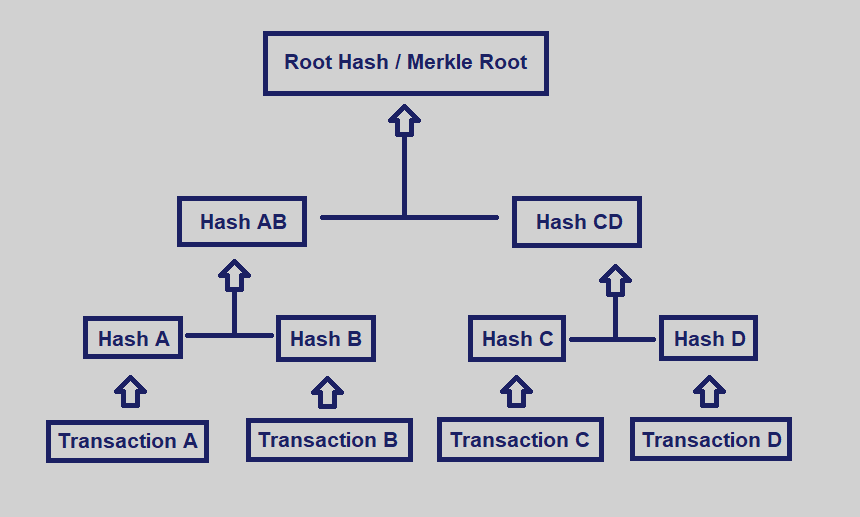
\includegraphics[width=0.7\linewidth]{images/merkle-tree.png}    

    \caption{
        The Merkle tree structure within a block of transactions. Transactions are hashed together as leaf nodes
        and repeated all the way up the tree to the main hash of the block, known as the Merkle root.
    }

    % use the notation fig:name to cross reference a figure
    \label{fig:merkle} 
\end{figure}

\section{Bitcoin and Cryptocurrency Technologies}
A large source of the information used to plan this project and choose the relevant technologies to include was the
book \emph{Bitcoin and Cryptocurrency Technologies} by Narayanan et al. This provided a more in depth disscussion
about the intricacies of the structures needed for the project. The book also gave good information about cryptocurrencies
that were not Bitcoin which gave a bigger picture and provided options for doing things differently or ways to 
exclude areas of bitcoin that would not be relevant in the project.

\subsection{Flooding}
%**
One of the key topics described in the book was the way for the nodes in the network to reach a consensus. This happens
multiple times during the running of a network. *** Once when nodes must identify and decide on which blockchain to use when
alternates appear. This is described by the Bitcoin white paper by picking the longest chain and distrobuting this to 
other nodes. It also happens when a new transaction occurs between two wallets, the transaction must be sent to all
nodes in order for the nodes to include it in their blocks so they can start mining the blocks to validate the transaction 
on the blockchain.

This method of flooding is explained in the book by showing that every node has a list of nearby nodes that is created
when it joins the network. Whenever a node recieves a transaction it first performs some checks and if it passes the 
checks, the transaction is propogated to all nodes on its nearby nodes list. First, the node checks if the transaction is
valid. It runs through the blockchain and checks that the funds the sender is trying to send actually belong to the sender.
Next, the node checks that the coins are not being double-spent, meaning the same funds have not already been sent to another
address perviously. Finally, the node checks if it has already seen the transaction and if it has, it just disgards this new
transaction as the node will already have added it to a block. If the transaction passes all these test it is sent to the
nearby nodes where it is put through the same tests until eventually it is spread to every node in the network or included
in a block on the blockchain.

\subsection{Mining}
One functionality described in the book is how mining changes over time. When a node mines a block that is included in the
blockchain they recieve a small reward which is an incentive to keep the blockchain updated. As explained perviously,
mining is the process of solving a hash calculation to result in a number starting with a certain number of '0's. The number
of 0s or target range, is changed over time. In Bitcoin, once every 2016 blocks that are mined the difficulty of mining will be
altered. The way that this difficulty is altered depends on how quickly blocks were mined in the previous 2016 blocks. This
is done in order to maintain a consistant mining speed. The faster the nodes are mining blocks, the harder the difficulty
will subsequently become. As the network of users increases, the processing power increases and so the mining will happen
faster. This is also offset as over time the size of the incentive reward for successfully mining a block is lowered.
This reward system is the only way new coins are created and because of this there is a maximum to the total amount of coins
that will be in the system. This effectivly makes Bitcoin immune to inflation.

The way bitcoin automatically responds to changes in the amount of processing power and size of the network is impressive,
however will not be a useful addition to the project. As this project will run at a relativly small scale over a small
time span, it would not be utilised and would be unnecessary to include this feature.

\subsection{Bitcoin scripting}
Another major part of blockchain that the book describes is the small scripting languague that was invented specifically for
transactions which helps with the verification of transfers. This simple bitcoin scripting language is used
by nodes when mining blocks to verify that all transactions in the block are valid. Every transaction in Bitcoin is
sent with a script, most often instructing the node to compute the inputs of this transaction and the specified outputs of
previous transactions to make sure they match up correctly. Bitcoin also utilises this scripting language to inform the node
what the output should equal when the receiver tries to verify the transaction signature using their key. The book goes
into detail about the intricacies of the language but this is out of scope for this project because including this scripting language
in the project would be unnecessary as there would only be one script needed and this can be implemented without the script.


%==================================================================================================================================
\chapter{Analysis/Requirements}
In this section we outline the exact nature of the project and how we gathered these requirements in order to 
complete the goals listed previously. We also discuss any functionality or features that have deliberatley been
left out of scope.

In this project the MoSCow method was used in order to prioritise the features so that the most important attributes
were included and some of the less important ones could be left to the end of the project to be added in if there was
time to spare.

\section{Functional Requirements}
Functional requirements listed here are features that must be included in the project in order for a woking,
useable cryptocurrency to be created. Without these requirements being met it would be impossible to carry out any
useful form of evaluation.

\subsection{Must have}
\begin{itemize}
    \item As described in the goals for the project, it would not constitute a cryptocurrency if it did not include a tamper-proof
        ledger for keeping track of all transactions between users. This must be resistant to malicious retroactive alterations
        and transactions that are invalid. This means that it must also have a feature so that nodes can run through the 
        whole chain and check all transactions are valid and each block links to the previous block.

    \item The cryptocurrency must also include some form of consensus mechanism where nodes can agree upon the blockchain
        and decide which transactions to include on the blockchain. They must be able to circulate each transaction once
        it occurs and flood it to other nodes on the network.
    
    \item Before blocks can be added to the blockchain it is important to inculde proof of work so that the integrity of the 
        networks blockchain can be maintained and guided by the processing power of the whole network and not a small minority
        of harmful nodes trying to take over.
\end{itemize}

\subsection{Should have}

A feature that can help with the smooth running of the network is an incentive for nodes to mine blocks. Without this there
is no reason for nodes to mine blocks and add to the blockchain. This is necessary as there needs to be a majority of 
honest nodes othewise it is easy for malicious nodes to take control of the blockchain and can then add any blocks with
which ever transactions they would like to the blockchain wether they are valid or not.

\subsection{Could have}
In Bitcoin, every 2016 blocks that are mined the difficulty of mining is changed in order to maintain the same average time
to mine a block. This difficulty is either made harder or easier based on how quickly the nodes mined the previous blocks.
This is not a high priority in this project as all the mining is taking place on the same computer and each node will have
the same computational power. In theory this means that the average time for mining blocks shouldn't change.

\section{Non-Functional Requirements}
Non-functional requiremnts are features that if included will improve the way the cryptocurrency operates by increasing
speed or lowering the storage space required. These features are not imperative to the operating of the cryptocurrency
but would bring the project closer to what might be used in current cryptocurrencies in the world at the moment.

\subsection{Must have}
It is important that the way in which the transactions within blocks is efficient. The must be stored using the Merkle
tree structure (REFERENCE). This way each transaction is a leaf node and every branch node is a hash of its two children.
This makes it extremely efficient for checking the validity of each block as you only have to check the hash of the root
hash.

\subsection{Should have}
The cryptocurrency should have the ability to split the balance of wallets such that if you send an amount but you only
have an increment of the currency larger than that amount then you should be sent back the value that you overpaid by.
For example if you start with 10 coins and you want to send 3 to another wallet you should be able to send your 10 coins
and recieve 7 back as overpay.

\subsection{Could have}
One feature that would save storage space would be the way in which transactions are stored in blocks. In the merkle tree
structure the transactions are hashed in order to speed up validation for nodes. This could be improved even more for 
nodes. It is possible that nodes only need to store the root hash of each block in order to do their validation as the
block hash is sufficient to check for incorrect transactions. This means each node can save a huge amount of storage space
by only storing each blocks root hash.

\section{Chosen Limitaions}
In this section some of the limitations that have been placed on the project which would not help demonstrate the 
primary purpose of the project are presented.
\begin{itemize}
    \item One feature that has been omitted is the concept of scripting. In Bitcoin, every transaction is sent
        with a short piece of code writen in the Bitcoin scripting language. This serves the function of allowing 
        different forms of transactions like ESCROW or multi user transactions. While useful in the functionality of
        Bitcoin, this feature is not necessary in our implemtation of a cryptocurrency as there will only be a need
        for one type of transaction.
    \item Another aspect chosen to exclude is the way in which nodes work. In real cryptocurrencies if a node
        has not been active in mining or creating transactions, after a specified amount of time the node will expire
        meaning other nearby nodes will cease to send transactions to this node. This effectivly removes the node from
        the network. This functionality is useful in keeping the list of nodes exclusive to active nodes and saves
        collective processing power for the whole network. In the project's implementation this would be unnecessary as a fixed
        number of nodes will be created for demonstration perposes.
\end{itemize}

%==================================================================================================================================
\chapter{Design}
In this section the decisions that were made when designing the project in order to meet the requirements
that have been laid out in the previous section are disscussed. The discussion will include the approach taken when
choosing one particular design instead of another and why those choices were made.

\section{Overview}
The main aspects of the design process that needed to be addressed were transactions, the blockchain, and
the consensus mechanism. It was also necessary to decide how all of these data structures would be linked together and
how the overall process of sending currency from one wallet to another would work between these structures.

%Maybe a system diagram showing how the structures interact

\section{Transactions}
%Structure and values
A transaction object is the basic building block of the whole cryptocurrency. This means that it must be designed 
to be secure and robust. Transactions should contain metadata that is able to identify and validate itself when
recieved and also contain the necessary information such as the amount of currency being sent in that transaction.

\subsection{Inputs and Outputs}
In order for a user to send some currency to another user they first have to have a sufficient amount themselves. The
way this condition was enforced was through the use of Transaction Inputs and Outputs. When a transaction is
sent, the value of that transaction (amount of currency it is attempting to send), is a collection of inputs. These inputs
are made up of the outputs of previous transactions that have been addresed to the user. This means that the process of
checking a user's balance would involve going through the blockchain adding up all the transaction outputs that
are addressed to that particular user and not already spent. This concept will be explained in more detail in the Blockchain section.

\subsection{Process and Checks}
%signatures
A key functionality of a transaction is it's ability to generate a signature for itself using the values
from the various metadata it contains. It also has to be able to vefify that this signature is valid.

%Process transaction
When a transaction is created it has to be processed before it is considered valid and added to a block and subsequently
the blockchain. This is done using a series of checks. The first check that the transaction makes is that the
signature is valid. This is paramount as it is one of the base functions that maintain the security of the 
cryptocurrency. Without this signature check it may be possible for one user to spoof the origin of a transaction
and send someone else's currency to themselves. The next step is to add up all the transaction inputs
and make sure that this is greater than or equal to the value of the transaction.

Once these checks have been completed it is time to execute the transaction. The way this is achieved is by
creating a new Transaction Output addressed to the recipient using the value of the transaction. It is important
that the previous transaction inputs are then removed as otherwise they would still be valid for the user to send
running the risk of double spend attacks. This is covered in more detail in the Blockchain section.

%Overpay
\subsection{Overpay}
In a real environment it is common that the ammount a user is trying to send is not equal to the value of one of
the transactions they have recieved in the past. For example, if a user recieves a transaction of 10 it is likely
that the next time they want to pay someone they may want to only send 5. This issue is solved by the concept of
overpay. In this design, when a user is sending a value to a recipient which is not equal to the transaction
input they are expending, the transaction processing creates two transaction outputs. The first sends the value
of the transaction to the recipient and the second sends the transaction input value minus the transaction value
back to the sender. This ensures that the transaction input is used up but the sender is not out of pocket.



%Coin creation
\subsection{Coin Creation}
When a transaction is created it can be one of two types. The first type is that of a normal transaction which would take place
between one wallet and another. The second type is that of coin creation. A transaction can be created with the 
coin creation flag which means that the inputs to the transaction would not contain anything but the transaction
would still be considered valid. This would only occur in the scenario like the very first transaction for the entire
cryptocurrency or the more frequent scenario which happens when a block is mined. To keep the system of consensus 
running there has to be an incentive for mining blocks. When a node mines a block they are rewarded with a small
amount of the currency which does not come from any particular user, instead this comes from a transaction with the
coin creation flag. After the initial creation of the network this is the only case where new currency will be
minted.

%Diagram of a transaction

\section{Blockchain}
The second major feature of the project to design is the Blockchain. This chain of blocks needs to be robust in
the sense that a malicious user cannot alter any previous transactions in the ledger for their benefit. It must
also be an accurate ledger containing every transaction exchanged to date. The way this blockchain was created was
by first collating a group of transactions into blocks. Then each block would create a signature hash which would
be a combination of all the transactions in the block. Then, in order to create an irreversible and immutable chain
of these blocks, the hash of each block is concatenated with the hash of the previous block in the chain. Meaning
any change to a transaction would cascade through each hash in each block and ultimately affect everything in the
chain. This means that it is easy for any node to check that the blockchain is valid using a simple and fast check.

%Blockchain diagram


\subsection{UTXOs}
The strategy of utilising Transaction inputs and transaction Outputs means that it is vital that the Blockchain
keeps track of the transaction outputs. When a user sends currency to another user, it is vital that the previous 
transaction output that the user has now spent, is removed. This is necessary for a few reasons, 
firstly if a user wants to find out how much currency they own they need to sum all the transaction outputs that 
are addressed to them. If the transactions are not tracked by removing transactions that are already spent, the 
user may be able to spend more than they own using double spending attacks.

This leads to the concept of an Unspent Transaction Output list (UTXO). This list is a structure tied to the blockchain
that stores all the transaction outputs that have not been spent as inputs by a tranasction. When they are used.
The transaction processing stage removes that output from the UTXO list and adds the new output to the list.
It is important to note that this is not a list of new transaction ouputs as that would not be secure outside the
blockchain and would be vulnerable to attack. It is simply a way of listing the transactions already added to the
blockchain. When a transaction is processed it goes through the new block and updates the UTXO list by recreating 
it. This maintains security and prevents malicious users from attacking the system this way.

\subsection{Block Structure}
%reference the previous diagram
The way the storage of transactions inside blocks was decided was using the same method utilised by Bitcoin using
Merkle trees. As mentioned earlier in this paper, a Merkle tree is a type of binary tree where each leaf node
is a transaction and each branch node is a hash of its two children. It was decided this would be the most effective
way of storing the transaction for this method as it would allow efficient and cheap validity checks for nodes
when testing the correctness of the blockchain. As this project is being designed to run on a test harness on one
machine it is important that the nodes be able to perform checks as quickly as possible.

%block size
Another important factor was the number of transactions to include in a block. The larger this number is, the
longer it will take to fill up with transactions and so the longer it will take I decided to keep the 
number of transactions in blocks relativly small in order to progress through the cryptocurrency lifecycle
more quickly and demonstrate all features.

\section{Consensus}
This final section dicusses the way in which the system was designed in order that all nodes communicate correctly and
that they all maintain an up-to-date copy of the blockchain. It also explains the decision to 
use one particular method of mining instead of alternatives.

\subsection{Proof of Work vs Proof of Stake}
In order for the network to function correctly, a consensus must be achieved by all the nodes. They need to agree
on what the correct blockchain is so they can add to it and they must also keep a consistant list of all the 
transactions yet to be included on the chain. It is vital that this consensus is achieved by nodes that are not
malicious or compromised and that the consensus they come to is proposed by an honest node to avoid attackers
taking over the blockchain. 

There are two common methods of distributed consensus methods. Proof of Work and Proof of Stake. These methods
are a way for nodes to prove that they are not malicious and are simply trying to honestly contribute to the
network. These concepts are not limited to cryptocurrencies and have many other applications in the world that 
have been researched by others [1,2]. The main idea behind these methods is tying the task of adding blocks to the 
blockchain to a reasouce that cannot be monopolised and as such the whole network cannot be controlled by a 
singular entity. Each method aims to achieve this in a different way by using different resources.

\subsubsection{Proof of Work}
This approach is the method that Bitcoin and most other cryptocurrencies use today. The resource it uses to 
ensure honesty is computational power. This means that in order to create a new block, a node has to demonstrate
that it has expended a certain amount of computational power. The way this is achieved is using hash calculations. 
This works by having a node take the previous block's
hash and the hash of the current block concatenated together with a number known as a nonce, resulting in a number
that falls within a specific target range. Nodes must go through incrementing the nonce in order to find the 
correct value that will satisfy the requirement. The size of the target range influences how hard and so how long
it will take for nodes to find. Once a node has found a nonce that results in a value inside the target range
they have proven that they have used compuational power and are entitled to add to the blockchain.

\subsubsection{Proof of Stake}
Much like the proof of work method, proof of stake is essentially assinging nodes the power to vote on what the
blockchain should be. The more of a resouce a node has, the more voting power it has. Proof of Stake is different
to Proof of Work as instead of tying voting power to computational power, it ties voting power to the amount
of currency a node holds. This means that the nodes with the most currency hold the most power to decide what the
blockchain will look like. In practice this means that these rich nodes will more often be selected to add a new
block to the chain. This methods has many advantages over the proof of work concept. This would significantly
reduce the environmental impact of the whole currency as there would be little to no mining taking place and so
there would be no groups of computers solving calculations indefinitely. This has the added benifit that
it would lower the chance that the network would become more centralised by mining companies. This method also
avoids the risk of a majority of malicious nodes aiming to destroy the currency. As any user holding any amount
of the currency is essentially a stakeholder in the network, any node that achieves a majority of the currency 
would have the ability to alter the course of the blockchain. With this method however, it would be in the best
interest of the majority stakeholder of the currency to perform honest actions as that would increase the value
of their currency.

In this project I have chosen to use the Proof of Work system as despite the real world benefits, like environmental
welfare, the proof of stake method does not present advantages when using a scale such as that being implemented
in this project. It would be more beneficial to show the proof of work system as mining would demonstrate the
functionality of the system better.

In this cryptocurrency the target range will be a number that begins with a certain
ammount of 0s. This means I have the ability to adjust the difficulty of the mining process by increasing
or decreasing the number of 0s in the target range. The more 0s required means that the final value must be more
specific and as such will take longer to find. I have decided that for this cryptocurrency the difficulty of mining
will remain low as processing power comes at a premium for one computer running multiple nodes.

\subsection{Nodes}
%Nearby nodes
In order for nodes to be able to communicate the details of transactions and the correct blockchain to use,
they first have to be able to identify and keep a list of nodes that are nearby in the network. This does not
necessarily mean geograpihcally nearby but in practice it is most likely nodes created most recently.
The way nodes are designed in this project is that a node is created with a seed node. Upon creation, nodes
query the seed node in order to obtain a list of nearby nodes, these nodes are selected randomly in order
to avoid every node's nearby list containing the same subset of the network.

%Transaction Flooding
\subsubsection{Transaction Flooding}
In order for nodes to mine blocks, they first have to know what transactions to include in the blocks. To do
this they need to know what transactions have occurred that are not currently included on the blockchain. This
is achieved by transaction flooding. When a transaction is created by a wallet it is sent to the node that the
wallet is associated with. This node then performs some checks on the transaction. The initial check is to make
sure that the transaction fits with the blockchain. It runs through all the inputs that the transaction claims
to be spending and makes sure that they line up with transaction outputs listed on the UTXO to make sure they
exist and haven't already been spent. The second check is to see if the transaction has already been seen by
the node if so it moves on without adding it to the block it is trying to create. If the transaction passes
these tests then the node adds it to the block it is planning to mine and then sends the transactions on to all
other nodes on its list of nearby nodes. Nodes recieving transactions like this from other nodes will perform the
same checks and then decide whether to pass on the transaction again. This way the transaction should be flooded
through the whole network and be eligable to be added to any block.

\subsection{Wallets}
%Something about wallets, maybe the overall process of sending coins
The design for wallets in this project is that every transaction must be tied to a wallet and every wallet
must be created from a node. This way, when a wallet creates a transaction it is automatically sent to the
associated node and can be flooded to the network. Each wallet has a public key which is used as the address
for which currency can be sent to and a private key which is used to verify each transaction. The wallets 
keep track of their own currency by running through the blockchain and adding up every transaction output
that is addressed to themselves. Even if a wallet spends some currency and then tries to spend the same
currency before the previous transaction is added to the blockchain it will be caught by the nodes before the
transaction will be flooded to prevent double spending attacks.

\section{Test Harness}
%Describing how the whole process works together
%Can include diagram showing main program flow
The final stage to designing the project was deciding how all of these features of the currency could be shown
and how the security could be effectivly presented. To meet the requiremnets specification it would mean developing
a test harness that could generate multiple nodes and simulate a real network of sending transactions back and 
forth between wallets in order to demonstrate the building of blocks and the blockchain. All while Demonstrating
the prevention of doubling spending and other attacks. 

\section{Chosing a Programming Language}
%Explain why object oriented programming was necessary 
%Explain why java for security packages etc
In order to decide what language we would use for this project it was best to look at how the project was designed
and then narrow it down to the most suitable contenders. The way in which this cryptocurrency was designed was 
utilising many different objects and structures, transactions, blocks, and the blockchain. This made it clear that 
the best choice of language for the project would be an object-oriented programming language. This narrowed down
the playing field to \textit{Java} or \textit{C\#}. From this it was decided that \textit{Java} would be the best 
option as it includes security packages which would be invaluble for implementing core features like signatures and 
public/private key verification.

\section{Summary}


%==================================================================================================================================
\chapter{Implementation}
This section of the paper will go in depth into the technical construction and implementation of the cryptocurrency.
This will start with describing the software development process used during construction and then how the different
aspects of the project were created and joined to deliver the finished product. This section will also examine the 
technical achievements made and how any problems that came to light were tackled.

%Show hashing equation
%Block mining specifics
%How the merkle trees worked
%UTXO hashmap
%Why blockchain is an arraylist
%Genesis blocks
%Finding nearby nodes

%Challanges and how they were overcome
%What did you do to implement this idea, and what technical achievements did you make?
%You can't talk about everything. Cover the high level first, then cover important, relevant or impressive details.

\section{Software Engineering Practices}
In order to create this cryptocurrencies it was important to have a solid software development process and an
aim to stick to the different practices.

\subsection{Version Control}
It was decided that the method of version control to be used would be Git. Making use of the GitHub website to 
host the project repository online. This allowed for the addition of code from different computers during the
development stages. This project made use of the branching feature of git in order to keep the project organised.
Every new feature/element that was added was designated a new branch and once complete was merged back into the
main development branch. Only at the end of the project was everything merged back into the master branch. This
was decided as the master branch is always supposed to keep a working copy of the software but this working copy
would not exist until the very end of the project as all the features had to be completed in order to work together
correctly. This was also the reason why the decision to not make use of continuous integration was made. It was
much faster and easier to run small tests and log outputs locally rather than make use of \textit{TravisCI} or an 
alternative.

GitHub was an incredibly important website to the construction of this project as it allowed the ability to keep
track of the completion of each feature using issues and milestones. Each feature and even small bugs were assigned
an issue [\ref{fig:issues}] and then those issues were assigned to one of the milestones [\ref{fig:milestones}]. 
This made it easy to prioritise each feature and keep on track with what needed to be done. The ritual of creating
an issue when a feature or problem is identified and then closing the issue when it is dealt with was important to 
the smooth development process.

% Issues Screenshot
\begin{figure}[!ht]
    \centering
    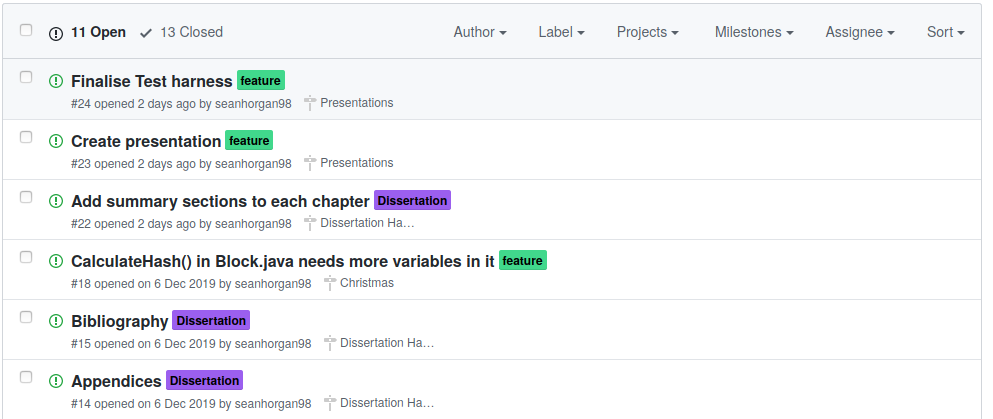
\includegraphics[width=1\linewidth]{images/issues.png}    

    \caption{
        A view of the main issue tracking board on GitHub. Making it easy to keep track of state of the project
        and what is still left to be completed.
    }

    % use the notation fig:name to cross reference a figure
    \label{fig:issues} 
\end{figure}
\vspace{10cm}

% Milestones screenshot
\begin{figure}[!ht]
    \centering
    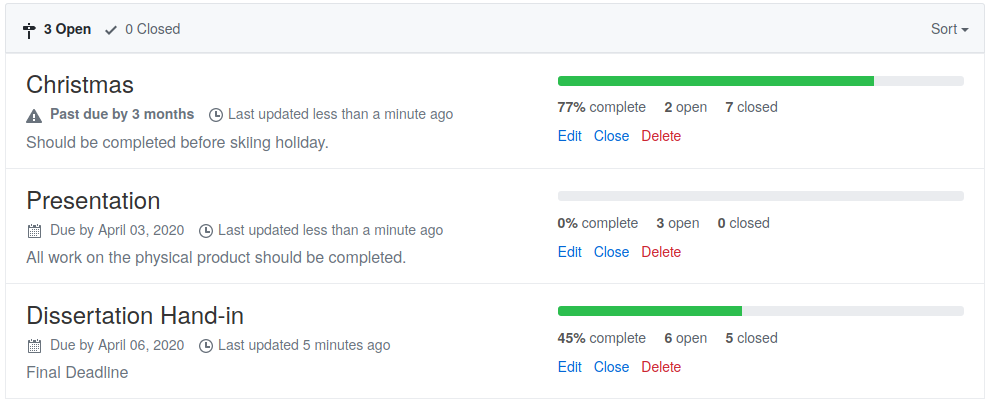
\includegraphics[width=1\linewidth]{images/milestones.png}    

    \caption{
        The main milestone board on GitHub showing the dates that each feature need to be completed by and
        allows for easy prioritisation of issues.
    }

    % use the notation fig:name to cross reference a figure
    \label{fig:milestones} 
\end{figure}

%Include images of issue boards and milestones etc

\section{Project Strucutre}
%Separation into classes and the string util class(will be talked about later), main

\section{Java security (String Util)}
%Signatures

\section{Maintanence}
%Documentation
%Code cleanliness?


\subsection{Figures}
\emph{Always} refer to figures included, like Figure \ref{fig:relu}, in the body of the text. Include full, explanatory captions and make sure the figures look good on the page.
You may include multiple figures in one float, as in Figure \ref{fig:synthetic}, using \texttt{subcaption}, which is enabled in the template.

\clearpage

\subsection{Equations}

Equations should be typeset correctly and precisely. Make sure you get parenthesis sizing correct, and punctuate equations correctly 
(the comma is important and goes \textit{inside} the equation block). Explain any symbols used clearly if not defined earlier. 

For example, we might define:
\begin{equation}
    \hat{f}(\xi) = \frac{1}{2}\left[ \int_{-\infty}^{\infty} f(x) e^{2\pi i x \xi} \right],
\end{equation}    
where $\hat{f}(\xi)$ is the Fourier transform of the time domain signal $f(x)$.

\subsection{Algorithms}
Algorithms can be set using \texttt{algorithm2e}, as in Algorithm \ref{alg:metropolis}.

% NOTE: line ends are denoted by \; in algorithm2e
\begin{algorithm}
    \DontPrintSemicolon
    \KwData{$f_X(x)$, a probability density function returing the density at $x$.\; $\sigma$ a standard deviation specifying the spread of the proposal distribution.\;
    $x_0$, an initial starting condition.}
    \KwResult{$s=[x_1, x_2, \dots, x_n]$, $n$ samples approximately drawn from a distribution with PDF $f_X(x)$.}
    \Begin{
        $s \longleftarrow []$\;
        $p \longleftarrow f_X(x)$\;
        $i \longleftarrow 0$\;
        \While{$i < n$}
        {
            $x^\prime \longleftarrow \mathcal{N}(x, \sigma^2)$\;
            $p^\prime \longleftarrow f_X(x^\prime)$\;
            $a \longleftarrow \frac{p^\prime}{p}$\;
            $r \longleftarrow U(0,1)$\;
            \If{$r<a$}
            {
                $x \longleftarrow x^\prime$\;
                $p \longleftarrow f_X(x)$\;
                $i \longleftarrow i+1$\;
                append $x$ to $s$\;
            }
        }
    }
    
\caption{The Metropolis-Hastings MCMC algorithm for drawing samples from arbitrary probability distributions, 
specialised for normal proposal distributions $q(x^\prime|x) = \mathcal{N}(x, \sigma^2)$. The symmetry of the normal distribution means the acceptance rule takes the simplified form.}\label{alg:metropolis}
\end{algorithm}

\subsection{Tables}

If you need to include tables, like Table \ref{tab:operators}, use a tool like https://www.tablesgenerator.com/ to generate the table as it is
extremely tedious otherwise. 

\begin{table}[]
    \caption{The standard table of operators in Python, along with their functional equivalents from the \texttt{operator} package. Note that table
    captions go above the table, not below. Do not add additional rules/lines to tables. }\label{tab:operators}
    %\tt 
    \rowcolors{2}{}{gray!3}
    \begin{tabular}{@{}lll@{}}
    %\toprule
    \textbf{Operation}    & \textbf{Syntax}                & \textbf{Function}                            \\ %\midrule % optional rule for header
    Addition              & \texttt{a + b}                          & \texttt{add(a, b)}                                    \\
    Concatenation         & \texttt{seq1 + seq2}                    & \texttt{concat(seq1, seq2)}                           \\
    Containment Test      & \texttt{obj in seq}                     & \texttt{contains(seq, obj)}                           \\
    Division              & \texttt{a / b}                          & \texttt{div(a, b) }  \\
    Division              & \texttt{a / b}                          & \texttt{truediv(a, b) } \\
    Division              & \texttt{a // b}                         & \texttt{floordiv(a, b)}                               \\
    Bitwise And           & \texttt{a \& b}                         & \texttt{and\_(a, b)}                                  \\
    Bitwise Exclusive Or  & \texttt{a \textasciicircum b}           & \texttt{xor(a, b)}                                    \\
    Bitwise Inversion     & \texttt{$\sim$a}                        & \texttt{invert(a)}                                    \\
    Bitwise Or            & \texttt{a | b}                          & \texttt{or\_(a, b)}                                   \\
    Exponentiation        & \texttt{a ** b}                         & \texttt{pow(a, b)}                                    \\
    Identity              & \texttt{a is b}                         & \texttt{is\_(a, b)}                                   \\
    Identity              & \texttt{a is not b}                     & \texttt{is\_not(a, b)}                                \\
    Indexed Assignment    & \texttt{obj{[}k{]} = v}                 & \texttt{setitem(obj, k, v)}                           \\
    Indexed Deletion      & \texttt{del obj{[}k{]}}                 & \texttt{delitem(obj, k)}                              \\
    Indexing              & \texttt{obj{[}k{]}}                     & \texttt{getitem(obj, k)}                              \\
    Left Shift            & \texttt{a \textless{}\textless b}       & \texttt{lshift(a, b)}                                 \\
    Modulo                & \texttt{a \% b}                         & \texttt{mod(a, b)}                                    \\
    Multiplication        & \texttt{a * b}                          & \texttt{mul(a, b)}                                    \\
    Negation (Arithmetic) & \texttt{- a}                            & \texttt{neg(a)}                                       \\
    Negation (Logical)    & \texttt{not a}                          & \texttt{not\_(a)}                                     \\
    Positive              & \texttt{+ a}                            & \texttt{pos(a)}                                       \\
    Right Shift           & \texttt{a \textgreater{}\textgreater b} & \texttt{rshift(a, b)}                                 \\
    Sequence Repetition   & \texttt{seq * i}                        & \texttt{repeat(seq, i)}                               \\
    Slice Assignment      & \texttt{seq{[}i:j{]} = values}          & \texttt{setitem(seq, slice(i, j), values)}            \\
    Slice Deletion        & \texttt{del seq{[}i:j{]}}               & \texttt{delitem(seq, slice(i, j))}                    \\
    Slicing               & \texttt{seq{[}i:j{]}}                   & \texttt{getitem(seq, slice(i, j))}                    \\
    String Formatting     & \texttt{s \% obj}                       & \texttt{mod(s, obj)}                                  \\
    Subtraction           & \texttt{a - b}                          & \texttt{sub(a, b)}                                    \\
    Truth Test            & \texttt{obj}                            & \texttt{truth(obj)}                                   \\
    Ordering              & \texttt{a \textless b}                  & \texttt{lt(a, b)}                                     \\
    Ordering              & \texttt{a \textless{}= b}               & \texttt{le(a, b)}                                     \\
    % \bottomrule
    \end{tabular}
    \end{table}
\subsection{Code}

Avoid putting large blocks of code in the report (more than a page in one block, for example). Use syntax highlighting if possible, as in Listing \ref{lst:callahan}.

\begin{lstlisting}[language=python, float, caption={The algorithm for packing the $3\times 3$ outer-totalistic binary CA successor rule into a 
    $16\times 16\times 16\times 16$ 4 bit lookup table, running an equivalent, notionally 16-state $2\times 2$ CA.}, label=lst:callahan]
    def create_callahan_table(rule="b3s23"):
        """Generate the lookup table for the cells."""        
        s_table = np.zeros((16, 16, 16, 16), dtype=np.uint8)
        birth, survive = parse_rule(rule)

        # generate all 16 bit strings
        for iv in range(65536):
            bv = [(iv >> z) & 1 for z in range(16)]
            a, b, c, d, e, f, g, h, i, j, k, l, m, n, o, p = bv

            # compute next state of the inner 2x2
            nw = apply_rule(f, a, b, c, e, g, i, j, k)
            ne = apply_rule(g, b, c, d, f, h, j, k, l)
            sw = apply_rule(j, e, f, g, i, k, m, n, o)
            se = apply_rule(k, f, g, h, j, l, n, o, p)

            # compute the index of this 4x4
            nw_code = a | (b << 1) | (e << 2) | (f << 3)
            ne_code = c | (d << 1) | (g << 2) | (h << 3)
            sw_code = i | (j << 1) | (m << 2) | (n << 3)
            se_code = k | (l << 1) | (o << 2) | (p << 3)

            # compute the state for the 2x2
            next_code = nw | (ne << 1) | (sw << 2) | (se << 3)

            # get the 4x4 index, and write into the table
            s_table[nw_code, ne_code, sw_code, se_code] = next_code

        return s_table

\end{lstlisting}

%==================================================================================================================================
\chapter{Evaluation} 
%Results tables for different sized blocks
%Number of nodes changes
%Unit tests results using program
%Why a user study would not be useful maybe? (Ask Ron)

\section{Aims}
\begin{itemize}
    \item Aims
    \item Aims
    \item Aims
\end{itemize}

\section{Unit tests}

\section{Performance Evaluation}

\section{Requirements Validation}

\section{Limitaitons}

How good is your solution? How well did you solve the general problem, and what evidence do you have to support that?

\section{Guidance}
\begin{itemize}
    \item
        Ask specific questions that address the general problem.
    \item
        Answer them with precise evidence (graphs, numbers, statistical
        analysis, qualitative analysis).
    \item
        Be fair and be scientific.
    \item
        The key thing is to show that you know how to evaluate your work, not
        that your work is the most amazing product ever.
\end{itemize}

\section{Evidence}
Make sure you present your evidence well. Use appropriate visualisations, reporting techniques and statistical analysis, as appropriate.

If you visualise, follow the basic rules, as illustrated in Figure \ref{fig:boxplot}:
\begin{itemize}
\item Label everything correctly (axis, title, units).
\item Caption thoroughly.
\item Reference in text.
\item \textbf{Include appropriate display of uncertainty (e.g. error bars, Box plot)}
\item Minimize clutter.
\end{itemize}

See the file \texttt{guide\_to\_visualising.pdf} for further information and guidance.

\begin{figure}
    \centering
    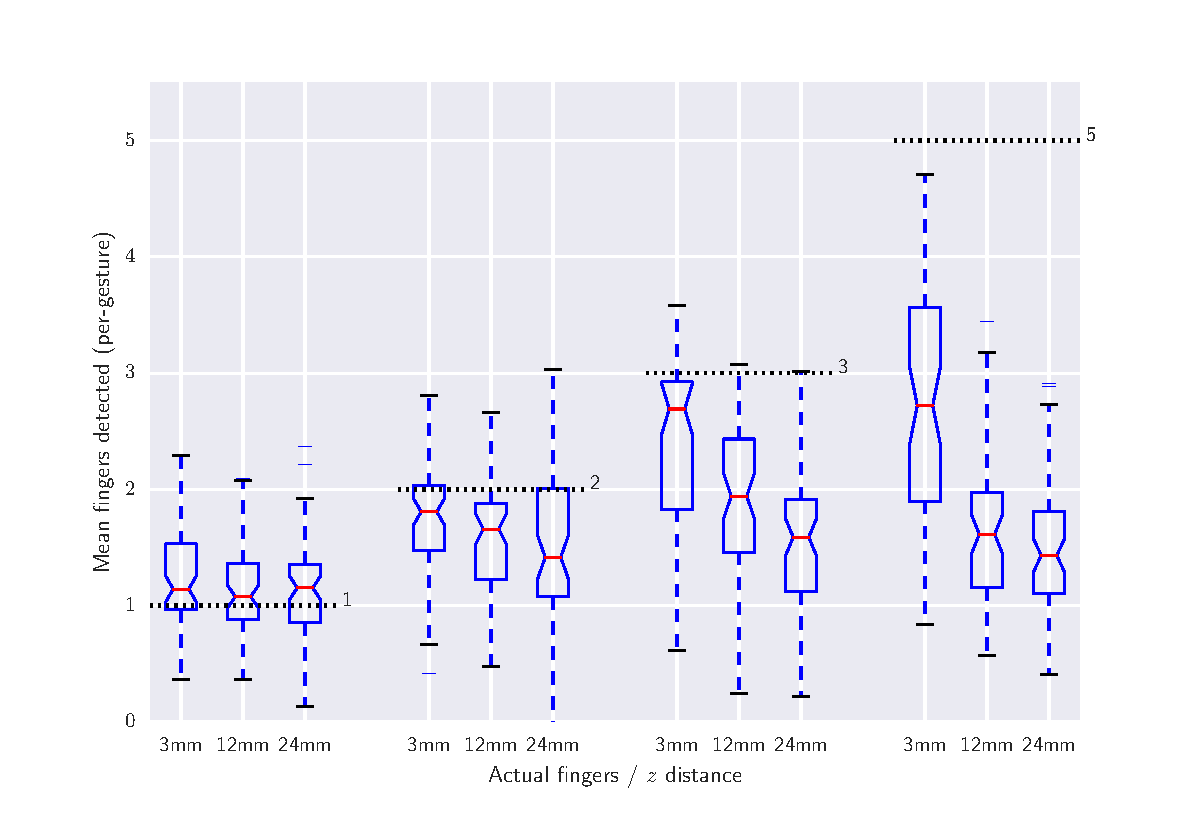
\includegraphics[width=1.0\linewidth]{images/boxplot_finger_distance.pdf}    

    \caption{Average number of fingers detected by the touch sensor at different heights above the surface, averaged over all gestures. Dashed lines indicate
    the true number of fingers present. The Box plots include bootstrapped uncertainty notches for the median. It is clear that the device is biased toward 
    undercounting fingers, particularly at higher $z$ distances.
    }

    % use the notation fig:name to cross reference a figure
    \label{fig:boxplot} 
\end{figure}


%==================================================================================================================================
\chapter{Conclusion}    
Summarise the whole project for a lazy reader who didn't read the rest (e.g. a prize-awarding committee).
\section{Guidance}
\begin{itemize}
    \item
        Summarise briefly and fairly.
    \item
        You should be addressing the general problem you introduced in the
        Introduction.        
    \item
        Include summary of concrete results (``the new compiler ran 2x
        faster'')
    \item
        Indicate what future work could be done, but remember: \textbf{you
        won't get credit for things you haven't done}.
\end{itemize}

\section{Future Work}

%==================================================================================================================================
%
% 
%==================================================================================================================================
%  APPENDICES  

\begin{appendices}

\chapter{Appendices}

Typical inclusions in the appendices are:

\begin{itemize}
\item
  Copies of ethics approvals (required if obtained)
\item
  Copies of questionnaires etc. used to gather data from subjects.
\item
  Extensive tables or figures that are too bulky to fit in the main body of
  the report, particularly ones that are repetitive and summarised in the body.

\item Outline of the source code (e.g. directory structure), or other architecture documentation like class diagrams.

\item User manuals, and any guides to starting/running the software.

\end{itemize}

\textbf{Don't include your source code in the appendices}. It will be
submitted separately.

\end{appendices}

%==================================================================================================================================
%   BIBLIOGRAPHY   

% The bibliography style is abbrvnat
% The bibliography always appears last, after the appendices.

\bibliographystyle{abbrvnat}

\bibliography{l4proj}
Merkle trees

Bitcoin white paper

Bitcoin and cryptocurrency technologies

https://hackernoon.com/merkle-trees-181cb4bc30b4
[IMAGE OF MERKLE TREE] 

\end{document}
